% This LaTeX was auto-generated from MATLAB code.
% To make changes, update the MATLAB code and export to LaTeX again.

\documentclass{article}

\usepackage[utf8]{inputenc}
\usepackage[T1]{fontenc}
\usepackage{lmodern}
\usepackage{graphicx}
\usepackage{color}
\usepackage{hyperref}
\usepackage{amsmath}
\usepackage{amsfonts}
\usepackage{epstopdf}
\usepackage[table]{xcolor}
\usepackage{matlab}

\sloppy
\epstopdfsetup{outdir=./}
\graphicspath{ {./lab1_wuqingy6_images/} }

\begin{document}

\matlabtitle{Introduction to Plotting and Vectorization}

\matlabheading{Student Information}

\begin{par}
\begin{flushleft}
Student Name: Qingyuan Wu
\end{flushleft}
\end{par}

\begin{par}
\begin{flushleft}
Student Number: 1007001664
\end{flushleft}
\end{par}

\matlabheading{Exercise 1}

\begin{par}
\begin{flushleft}
Objective: Observe a MATLAB error when you try to access an invalid index.
\end{flushleft}
\end{par}

\begin{par}
\begin{flushleft}
Details: Try to access elements of the vector \texttt{x}, created in the previous step at the command prompt \texttt{\textgreater{}\textgreater{}}. Try values of \texttt{i} outside the valid range. Try negative values, zero, and large positive values. Copy down the error message in each case, and report this in your submitted work as:
\end{flushleft}
\end{par}

\begin{matlabcode}
% Only include the error message as a comment (with the percent signs), 
% DO NOT INCLUDE THE CODE IN YOUR SUBMISSION.

% Error for negative index:
%   x(-1)
%   Array indices must be positive integers or logical values.

% Error for zero index:
%   x(0)
%   Array indices must be positive integers or logical values.

% Error for positive index outside of the bounds:
%   x(10)
%   Index exceeds the number of array elements (6).
\end{matlabcode}


\matlabheading{Exercise 2}

\begin{par}
\begin{flushleft}
Objective: Create two vectors and plot one against the other.
\end{flushleft}
\end{par}

\begin{par}
\begin{flushleft}
Details: Explicitly create the vectors 
\end{flushleft}
\end{par}

\begin{par}
\begin{flushleft}
x = [-5, -3, -1, 0, 2, 4, 6] 
\end{flushleft}
\end{par}

\begin{par}
\begin{flushleft}
and 
\end{flushleft}
\end{par}

\begin{par}
\begin{flushleft}
y = [-25, -9, -1, 0, 4, 16, 36]
\end{flushleft}
\end{par}

\begin{par}
\begin{flushleft}
And plot \texttt{x} against \texttt{y}. Your submission should show both the creation of the vectors and the figure, as in the example.
\end{flushleft}
\end{par}

\begin{matlabcode}
x = [-5, -3, -1, 0, 2, 4, 6]
\end{matlabcode}
\begin{matlaboutput}
x = 1x7    
    -5    -3    -1     0     2     4     6

\end{matlaboutput}
\begin{matlabcode}
y = [-25, -9, -1, 0, 4, 16, 36]
\end{matlabcode}
\begin{matlaboutput}
y = 1x7    
   -25    -9    -1     0     4    16    36

\end{matlaboutput}
\begin{matlabcode}
plot(x,y);
\end{matlabcode}
\begin{center}
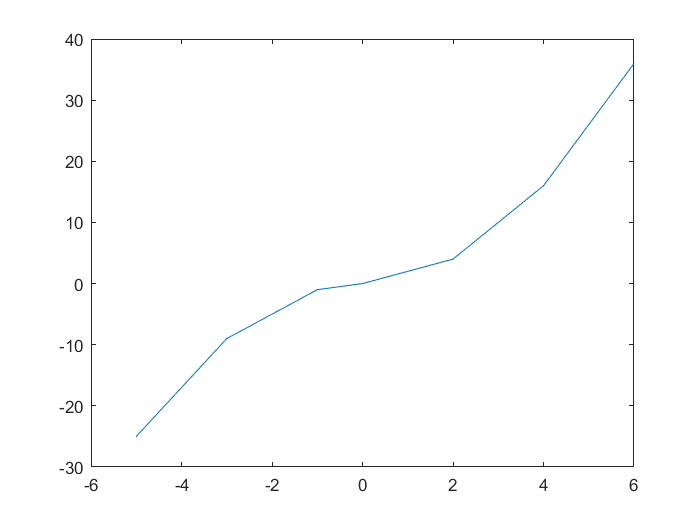
\includegraphics[width=\maxwidth{56.196688409433015em}]{figure_0.png}
\end{center}


\matlabheading{Exercise 3}

\begin{par}
\begin{flushleft}
Objective: Plot \texttt{x}.x
\end{flushleft}
\end{par}

\begin{par}
\begin{flushleft}
Details: Using a for loop, create a vector x of 101 equally spaced points between -3 and 7, inclusive. Then create a vector y, such that \texttt{y(i) = abs(x(i))*x(i)} using a for loop. Plot the results. 
\end{flushleft}
\end{par}

\begin{par}
\begin{flushleft}
Your submission should include the code, as in the example, and appropriate comments.
\end{flushleft}
\end{par}

\begin{matlabcode}
N = 101;

% preallocate x and y with zeros
x = zeros(N,1);
y = zeros(N,1);

% Variables for domain
start = -3;
endd = 7;

% calculate the increment
h = (endd-start)/(N-1);

% loop through to fill x and y values
for i = 1:N
    x(i) = start + h*(i-1);
    y(i) = abs(x(i)) * x(i); % modify the preallocated y array
end

plot(x,y); % plot the vectors as ordered pairs
\end{matlabcode}
\begin{center}
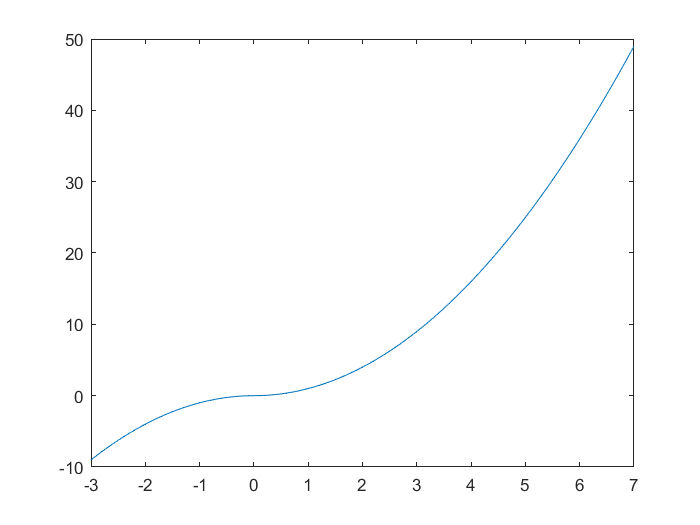
\includegraphics[width=\maxwidth{56.196688409433015em}]{figure_1.png}
\end{center}


\matlabheading{Exercise 4}

\begin{par}
\begin{flushleft}
Objective: Compare the speedup from vectorization for a larger vector.
\end{flushleft}
\end{par}

\begin{par}
\begin{flushleft}
Details: Create a vector \texttt{x} of 5000001 equally spaced points between -2 and 3, inclusive, using a for loop. Then time the construction of vector \texttt{y}, whose values are arctan of x, by a for loop and by vectorization. Be sure to clear  \texttt{y} between the two runs. (Hint: use the help file to find the command for arctan!)
\end{flushleft}
\end{par}

\begin{par}
\begin{flushleft}
Your submission should include the code, as in the example, with appropriate comments.
\end{flushleft}
\end{par}

\begin{matlabcode}
N = 5000001; % number of points to generate
start = -2; % interval is [-2, 3]
endd = 3;
h = (endd-start)/(N-1); % increment
x = zeros(5000001,1); % preallocate x with zeros

for i = 1:N % populate x
    x(i) = start + (i-1) * h;
end

tic % start timer
y = zeros(N,1);
for i = 1:N % generate y data using for loop
    y(i) = atan(x(i));
end
toc % end timer, display time
\end{matlabcode}
\begin{matlaboutput}
Elapsed time is 0.133264 seconds.
\end{matlaboutput}
\begin{matlabcode}

% "Elapsed time is 0.102163 seconds."

clear y;

tic % start timer
y = atan(x); % generate y data using vectorization
toc % end timer, display time
\end{matlabcode}
\begin{matlaboutput}
Elapsed time is 0.028637 seconds.
\end{matlaboutput}
\begin{matlabcode}

% "Elapsed time is 0.024718 seconds."

clear y;
\end{matlabcode}


\matlabheading{Exercise 5}

\begin{par}
\begin{flushleft}
Objective: Solve an ODE and plot three particular solutions.
\end{flushleft}
\end{par}

\begin{par}
\begin{flushleft}
Details: Manually find the general solution of the ODE:
\end{flushleft}
\end{par}

\begin{par}
\begin{flushleft}
dy/dt + (2*t)*y = 1/exp(t\textasciicircum{}2)
\end{flushleft}
\end{par}

\begin{par}
\begin{flushleft}
and the particular solutions for initial conditions y(1) = -1, y(1) = 0, and y(1) = 1. Plot these three particular solutions on the same axes lettting the independent variable range from 1 to 5. 
\end{flushleft}
\end{par}

\begin{matlabcode}
% general solution: y = (t+C)/exp(t^2), t = [1,5]
% y(1) = -1 => y = (t-e-1)/exp(t^2)
% y(1) = 0 => y = (t-1)/exp(t^2)
% y(1) = 1 => y = (t+e-1)/exp(t^2)

% Once you have the three particular solutions you will
% need to:
%
%  1. Create a vector for the independent variable, t.  Use linspace with
%  a reasonable number of points (100 is fine).
%  2. Create vectors for the three solutions.  Use vectorized operations.
%  3. Plot three solutions on the same axes, annotating the figure
%   appropriately.

% creating the t vector
t = linspace(1, 5, 100);

% creating the vectors for the particular solutions
y0 = (t-1)./exp(t.^2);
y1 = (t+exp(1)-1)./exp(t.^2);
y2 = (t-exp(1)-1)./exp(t.^2);

% plotting the particular solutions
plot(t, y0, t, y1, t, y2);

% labels and legend
xlabel("t");
ylabel("y(t)");
title("Particular Solutions to dy/dt + 2*t*y = 1/exp(t^2)");
legend("y(1)=0", "y(1)=1", "y(1)=-1");
\end{matlabcode}
\begin{center}
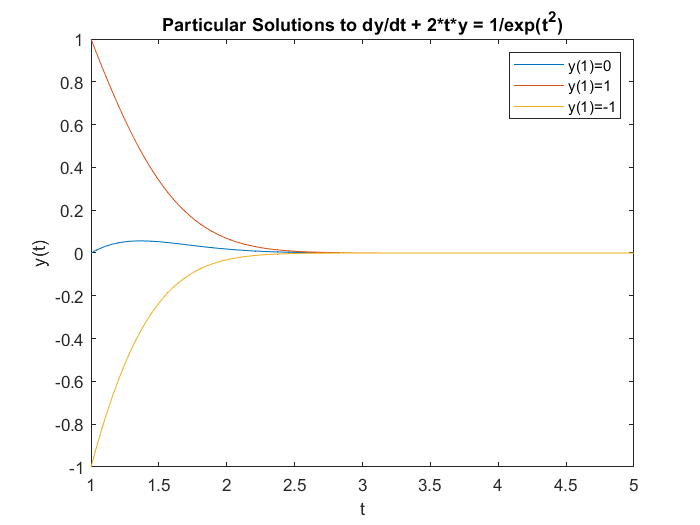
\includegraphics[width=\maxwidth{56.196688409433015em}]{figure_2.png}
\end{center}
\begin{matlabcode}
% Your submission should include, in the description section, the general 
% solution of the ODE and the three particular solutions.  It should also 
% have the appropriately commented code.
\end{matlabcode}


\matlabheading{Exercise 6}

\begin{par}
\begin{flushleft}
Objective: Write and use an inline function of one variable.
\end{flushleft}
\end{par}

\begin{par}
\begin{flushleft}
Details: Define the inline function for
\end{flushleft}
\end{par}

\begin{par}
\begin{flushleft}
\texttt{f(x) = (x\textasciicircum{}3 - abs(x)) * ln(x\textasciicircum{}2+1)}
\end{flushleft}
\end{par}

\begin{matlabcode}
% defining the function
f = @(x) (x.^3 - abs(x)) .* log(x.^2+1);

% compute f(0), f(1), f(-1)
fprintf("f(%g) = %g\n", 0, f(0));
\end{matlabcode}
\begin{matlaboutput}
f(0) = 0
\end{matlaboutput}
\begin{matlabcode}
fprintf("f(%g) = %g\n", 1, f(1));
\end{matlabcode}
\begin{matlaboutput}
f(1) = 0
\end{matlaboutput}
\begin{matlabcode}
fprintf("f(%g) = %g\n", -1, f(-1));
\end{matlabcode}
\begin{matlaboutput}
f(-1) = -1.38629
\end{matlaboutput}
\begin{matlabcode}

% 100 points in [-5, 5]
x = linspace(-5, 5, 100);

% plotting the function
plot(x, f(x), "b-");

% labels
xlabel("x");
ylabel("y = f(x)");
title("Graph of y = (x^3 - abs(x)) * ln(x^2+1)");
\end{matlabcode}
\begin{center}
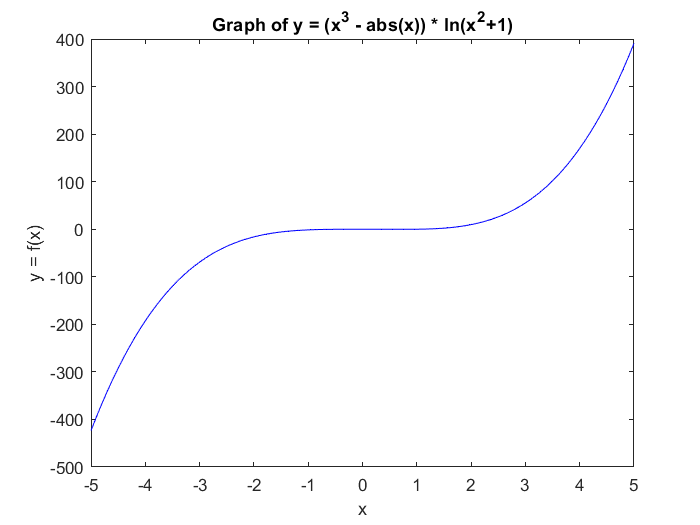
\includegraphics[width=\maxwidth{56.196688409433015em}]{figure_3.png}
\end{center}
\begin{matlabcode}

% Use this function to compute |f(0)|, |f(1)|, and |f(-1)| and plot the
% function with 100 grid points from -5 to 5. Make sure to
% use vectorization in your definition, and label your axes.
%
% Your submission should show the definition of the function, and the
% computation of these values.
\end{matlabcode}


\matlabheading{Exercise 7}

\begin{par}
\begin{flushleft}
Objective: Write and use an inline function of two variables.
\end{flushleft}
\end{par}

\begin{par}
\begin{flushleft}
Details: Define the inline function for
\end{flushleft}
\end{par}

\begin{par}
\begin{flushleft}
\texttt{f(x,y) = y + y\textasciicircum{}3 - cos x + x\textasciicircum{}2 - x\textasciicircum{}4}
\end{flushleft}
\end{par}

\begin{matlabcode}
f = @(x,y) y + y.^3 - cos(x) + x.^2 - x^4;

fprintf("f(%g, %g) = %g\n", 0, 0, f(0,0));
\end{matlabcode}
\begin{matlaboutput}
f(0, 0) = -1
\end{matlaboutput}
\begin{matlabcode}
fprintf("f(%g, %g) = %g\n", pi/2, 1, f(pi/2,1));
\end{matlabcode}
\begin{matlaboutput}
f(1.5708, 1) = -1.62067
\end{matlaboutput}
\begin{matlabcode}
fprintf("f(%g, %g) = %g\n", -1, -1, f(-1,-1));
\end{matlabcode}
\begin{matlaboutput}
f(-1, -1) = -2.5403
\end{matlaboutput}
\begin{matlabcode}
f(0,0)
\end{matlabcode}
\begin{matlaboutput}
ans = -1
\end{matlaboutput}
\begin{matlabcode}
f(pi/2,1)
\end{matlabcode}
\begin{matlaboutput}
ans = -1.6207
\end{matlaboutput}
\begin{matlabcode}
f(-1,-1)
\end{matlabcode}
\begin{matlaboutput}
ans = -2.5403
\end{matlaboutput}
\begin{matlabcode}
% Note that |f(x,y) = c| is the implicit solution to 
%
% |dy/dx = (4x^3 - 2x - sin x)/(1+3y^2)|.
%
% See Examples 1-3 of section 2.1 in Brannan and Boyce for similar examples.
%
% Use this function to compute |f(0, 0)|, |f(pi/2,1)|, and |f(-1,-1)|.  Make
% sure to use vectorization in your definition.
%
% Your submission should show the definition of the function, and the
% computation of these values.
%
\end{matlabcode}


\matlabheading{Exercise 8}

\begin{par}
\begin{flushleft}
Objective: Use fzero to solve an equation \texttt{f(x,y)=0} for y at different values of x.
\end{flushleft}
\end{par}

\begin{par}
\begin{flushleft}
Details: Consider the function
\end{flushleft}
\end{par}

\begin{par}
\begin{flushleft}
\texttt{f(x,y) = y + y\textasciicircum{}3 - cos x + x\textasciicircum{}2 - x\textasciicircum{}4}
\end{flushleft}
\end{par}

\begin{matlabcode}
% Define the inline function
f = @(x,y) y + y.^3 - cos(x) + x.^2 - x.^4;
x0 = 0;
guess = 0.5;
g = @(y) f(x0, y);
y = fzero(g, guess);
fprintf(' Solution for x = %g: y = %g\n', x0, y);
\end{matlabcode}
\begin{matlaboutput}
 Solution for x = 0: y = 0.682328
\end{matlaboutput}
\begin{matlabcode}

fprintf('---------------------------\n');
\end{matlabcode}
\begin{matlaboutput}
---------------------------
\end{matlaboutput}
\begin{matlabcode}

y0 = 1/2;
h = @(x) f(x, y0);

guess = 1;
x = fzero(h, guess);
fprintf(' Solution for y = %g: x = %g\n', y0, x);
\end{matlabcode}
\begin{matlaboutput}
 Solution for y = 0.5: x = 1.05844
\end{matlaboutput}
\begin{matlabcode}

guess = 0.5;
x = fzero(h, guess);
fprintf(' Solution for y = %g: x = %g\n', y0, x);
\end{matlabcode}
\begin{matlaboutput}
 Solution for y = 0.5: x = 0.567406
\end{matlaboutput}
\begin{matlabcode}

% Define the appropriate inline function and compute the single solution 
% at |x = 0| and the two positive solutions at |y = 1/2|.  
%
% You will need to experiment with different guesses to get these three
% solutions.
%
% Your submission should show the definition of the function, and the
% computation of these three roots.
\end{matlabcode}


\matlabheading{Exercise 9}

\begin{par}
\begin{flushleft}
Objective: Plot a portion of an implicit equation.
\end{flushleft}
\end{par}

\begin{par}
\begin{flushleft}
Details: Plot the portion of the solution to
\end{flushleft}
\end{par}

\begin{par}
\begin{flushleft}
\texttt{f(x,y) = y + y\textasciicircum{}3 - cos x + x\textasciicircum{}2 - x\textasciicircum{}4}
\end{flushleft}
\end{par}

\begin{matlabcode}
xvals = linspace(-2, 2, 100);
yvals = zeros(100,1);

f = @(x,y) y + y.^3 - cos(x) + x.^2 - x.^4;
for j = 1:length(xvals)
   h = @(y) f(xvals(j),y);
   % solve the implicit equation:
   yvals(j) = fzero(h, 0.5);
end

% Plot the results
plot(xvals, yvals);

% labels
xlabel("x");
ylabel("y");
title("Solution to 0 = y + y^3 - cos x + x^2 - x^4 for x in [-2,2]");
\end{matlabcode}
\begin{center}
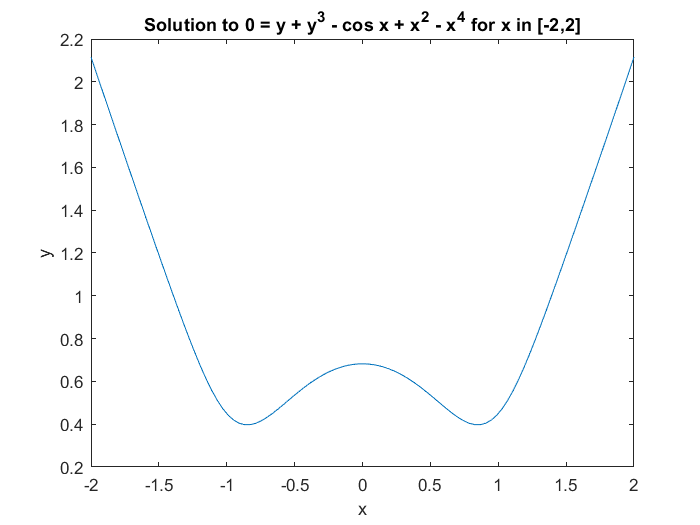
\includegraphics[width=\maxwidth{56.196688409433015em}]{figure_4.png}
\end{center}
\begin{matlabcode}

% passing through the point |(0,0)| for x from -2 to 2.  Use 100 grid
% points.
%
% You will need to be careful with the initial guess you use in solving the
% equation.
%
% Your submission should show the definition of the function, the
% construction of the arrays, the for loop, and the resultant figure.
%
% Label your axes.
%
\end{matlabcode}


\matlabheading{Exercise 10 - NOT FOR SUBMISSION}

\begin{par}
\begin{flushleft}
Objective: Solve a differential equation and plot a portion of it.
\end{flushleft}
\end{par}

\begin{par}
\begin{flushleft}
Details: Find the general implicit solution of the differential equation
\end{flushleft}
\end{par}

\begin{par}
\begin{flushleft}
\texttt{dy/dx = (-cos x + 3x\textasciicircum{}2) y} dy/y = (-cosx + 3x\textasciicircum{}2)dx \% integrate both sides: ln(y) = -sinx + x\textasciicircum{}3 + C y = A*exp(-sinx + x\textasciicircum{}3) y(0) = 1 =\textgreater{} A = 1 paricular sol'n: y = exp(-sinx + x\textasciicircum{}3)
\end{flushleft}
\end{par}

\begin{matlabcode}
% Plot the particular solution passing through y(0) = 1 using 100 grid
% points for x in [-1.5, 1.25].
%
% Be careful on your choice of guess. You will be penalized if MATLAB shows
% an error.
%
% Your submission should show the general and particular solutions, in
% implicit form, in the comments, the definition of the appropriate inline
% functions, arrays, the for loop, and the figure.
%
% Label your axes.
\end{matlabcode}


\matlabheading{Exercise 11}

\begin{par}
\begin{flushleft}
Objective: use iode a plot the direction field of a differential equation
\end{flushleft}
\end{par}

\begin{par}
\begin{flushleft}
Details: After starting iode, click the "direction fields" button from the main menu. The default is the direction field for
\end{flushleft}
\end{par}

\begin{par}
\begin{flushleft}
\texttt{dy/dx = sin(y-x)}
\end{flushleft}
\end{par}

\begin{par}
\begin{flushleft}
Click any point in the x-y plane to see a (numerically computed) solution to the differential equation passing through that point.
\end{flushleft}
\end{par}

\begin{par}
\begin{flushleft}
Starting from the "Equation" menu, plot the direction field of 
\end{flushleft}
\end{par}

\begin{par}
\begin{flushleft}
\texttt{dy/dx = xy\textasciicircum{}2}
\end{flushleft}
\end{par}

\begin{matlabcode}
% - Behaviour: all solutions are symmetric about the y-axis. Solutions with
% initial values above the x-axis tend to approach infinity. Solutions with
% initial values below the x axis tend to approach y=0.
% There is a semi-stable equilibrium at y=0:
% - As x approaches infinity, y approaches 0 for initial value <= 0; y
% appraoches infinity for initial value > 0.
% - The general solution to y' = xy^2 is y = -2/(x^2+C).
% From this we can conclude y(x) = y(-x) for all values of C. Therefore
% solutions to this ODE are symmetric about the y-axis.

% Describe, in words, the behaviour of the solutions. What happens as x
% approaches infinity? Explain why solutions are symmetric about the 
% y-axis, i.e. |y(x)=y(-x)| for any solution.
\end{matlabcode}


\matlabheading{Exercise 12}

\begin{par}
\begin{flushleft}
Objective: study the long-run behaviour of a differential equation from its direction field
\end{flushleft}
\end{par}

\begin{par}
\begin{flushleft}
Details: Using iode, plot the direction field of 
\end{flushleft}
\end{par}

\begin{par}
\begin{flushleft}
\texttt{dy/dx = y\textasciicircum{}4 - y\textasciicircum{}3 - 3*y\textasciicircum{}2 + y + 2}
\end{flushleft}
\end{par}

\begin{par}
\begin{flushleft}
By clicking on various initial conditions \texttt{y(0) = y\_0} (iode plots the solution), determine the long-run behaviour of solutions as a function of \texttt{y\_0}. In other words, list the constant solutions that are approached as x goes to infinity and how \texttt{y\_0} determines which constant solution is approached.
\end{flushleft}
\end{par}

\begin{matlabcode}
% If your numerically computed solutions ever appear to cross then change
% the solution method from Euler to the, much better, Runge-Kutta method.
% Think about why solutions are not permitted to cross. If they do then
% this indicates a problem with the numerical solver.

% Equilibrium:
% There are three equilibria in the direction field, y=2, y=1, and y=-1.
% y=2 is an unstable equilibrium because the solutions diverge from y=2 as
% x approaches infinity.
% y=1 is a stable equilibrium because the solutions approach y=1 as x
% approaches infinity.
% y=-1 is a semi-stable equilibrium because solutions with initial values
% less than -1 eventually approach -1, but solutions with initial values
% greater than -1 diverge from -1.

% From observations: y(x0) = 2 will make the solution stablize at y = 2
% y(x0) > 2 will make the solution blow up to infinity
% -1 < y(x0) < 2 will make the solution approach 1
% y(x0) = -1 will make the solution stablizie at y = -1
% y(x0) < -1 will make the solution approach -1
\end{matlabcode}

\end{document}
